\chapter{Chapter One}
\label{ch:chapter-one}
\lipsum[1-3]\cite{DUMMY:1}
\begin{figure}	
	\centering
	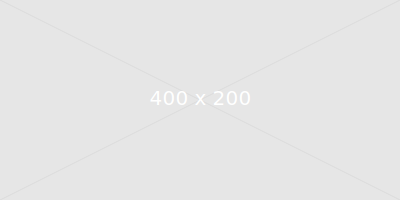
\includegraphics[width=\textwidth]{img/placeholder400x200}
	\caption{Sample figure.}
	\label{fig:sample-figure}
\end{figure}

\lipsum[1-3]\cite{DUMMY:2}

\begin{table}
	\centering
	\begin{tabular}{|c|c|c|}
		\hline
		Header-1 & Header-2 & Header-3 \\
		\hline\hline
		Content-1 & Content-2 & Content-3 \\
		\hline
		Content-1 & Content-2 & Content-3 \\
		\hline
		Content-1 & Content-2 & Content-3 \\
		\hline		
	\end{tabular}
	\caption{Sample table.}
	\label{tab:sample-table}
\end{table}

\lipsum[1-3]\cite{DUMMY:2}

\lstinputlisting[language=C,style=customc, caption={Sample code listing.}, label={cod:sample-code}]{code/hello-world.c}

\lipsum[1-3]\cite{DUMMY:3}



